\documentclass{article}
\usepackage{amssymb}
\usepackage[utf8]{inputenc}
\usepackage{geometry}
\usepackage{mathtools}
\usepackage{verbatim}

\geometry{letterpaper, portrait, margin=1in}

\title{CS325 - Project 2}
\author{Group \#6 \\ William Jernigan, Alexander Merrill, Sean Rettig}
\date{\today}

\begin{document}

\maketitle

\section*{Correctness}
\subsection*{Proof of Claim 3: ___ Proof}

\begin{quote}
Claim 3: If $\{z_{1},z_{2},...,z_{t}\}$ and $\{z_{1},z_{2},...,z_{s}^{'}\}$ are two visible sets of lines (each ordered by increasing slope), then the visible subset of $\{z_{1},z_{2},...,z_{t}\}\cup\{z_{1},z_{2},...,z_{s}^{'}\}$ is $\{z_{1},...,z_{i}\}$ for some $i \leq 1$ and $j \leq s$.
\end{quote}

\subsubsection*{Prove that $\{a_{1},...,a_{i}\}$ is visible}
    Because all elements in A were defined to be visible with respect to each other, any covering line $b_{q}$ must be from B.\\
    Given that $m_{a_{t}} < m_{b_{1}}$, a covered line $a_{p} \in A$ has $m_{p} < m_{q}$.
    
    \paragraph{Prove that for any covered line  $a_{p}, p = i + 1$, all lines to the right of p in A are also covered:}
        Because $a_p$ is defined to be invisible, then by Claim 2 in the P1 Visible Lines Handout:\\
        $y_{a_{p-1}}(x_{a_{p-1}, b_{q}}) > y_{a_{p}}(x_{a_{p-1},b_{q}})$, where $x_{a_{p-1}, b_{q}}$ is the x coordinate where $a_{p-1}$ and $b_q$ intersect.\\
        Because $a_{p+1}$ is defined to not cover $a_p$, we know that $y_{a_{p}}(x_{a_{p-1}, b_{q}}) > y_{a_{p+1}}(x_{a_{p-1},b_{q}})$.\\
        For $x < x_{a_{p-1},a_{p}}, a_{p+1}$ is covered by $a_p$.\\
        We need to show that $a_{p+1}$ is covered for $x \geq x_{a_{p-1},a_{p}}$.\\
        Because $b_q$ is covering $a_p$, $y_{b_{q}}(x) > y_{a_{q}}(x)$ for $x \geq x_{a_{p-1},b_{q}} \geq x_{a_{p-1},a_{p}}$.\\
        \therefore $p+1$ is invisible if p is invisible.\\
        This follows for all p.
Then let $p = i + 1$. \therefore $\{a_1,...,a_i\}$ is visible and $\{a_p,...,a_t\}$ is invisible.\\
Do the same thing for set B.


\subsection*{Proof of Algorithm 4: Inductive Proof}


\section*{Experimental and Asymptotic Run Time Analysis}
\subsection*{Experimental Run Time Data}
\verbatiminput{times.txt}

\pagebreak

\subsection*{Experimental Run Time Plots}
\centerline{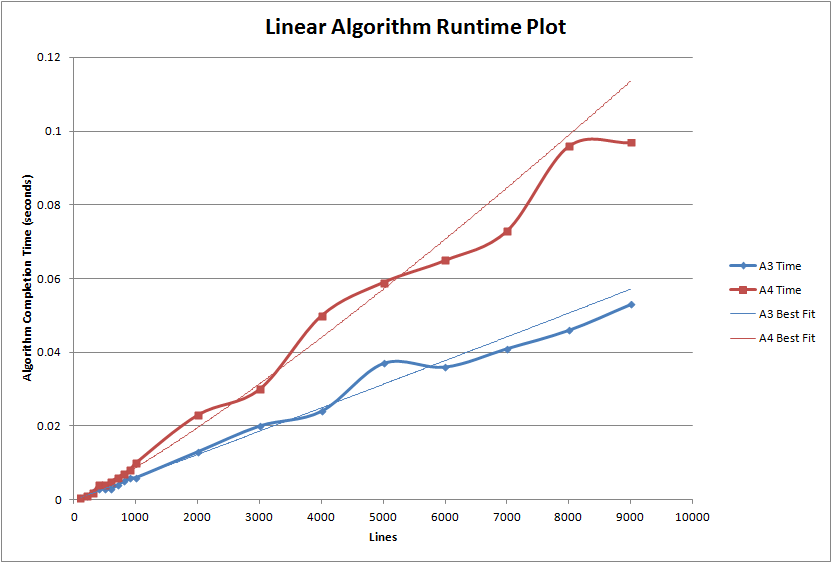
\includegraphics[width=0.75\textwidth]{plot1.png}}
\centerline{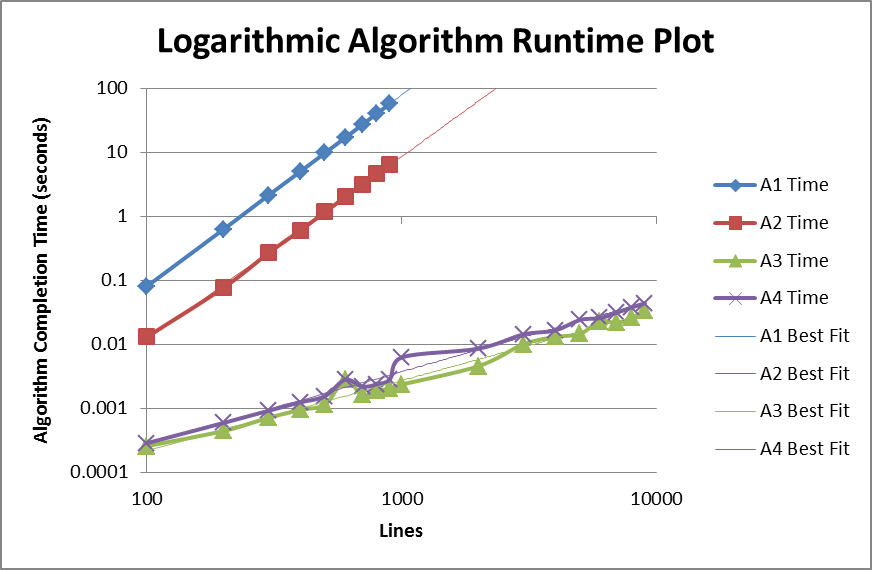
\includegraphics[width=0.75\textwidth]{plot2.png}}

\pagebreak

\subsection*{Experimental Run Time Analysis}
Algorithm 1: $y=8 \times 10^{-8}x^{3.0026}$\\
Algorithm 2: $y=4 \times 10^{-8}x^{2.7892}$\\
Algorithm 3: $y=7 \times 10^{-6}x^{0.8868}$\\
Algorithm 4: $$\\

Given these equations, we can use both the slopes and our code to analyze the run times of the algorithms.

\subsection*{Asymptotic Run Time Analysis}
Algorithm 1: $\Theta(n^3)$\\
Algorithm 2: $\bigcirc(n^3)$\\
Algorithm 3: $\bigcirc(n^2),\Omega(n)$\\
Algorithm 4: $\bigcirc(nlogn),\Omega(logn)$\\
\indent Algorithm 4 

\subsection*{Discrepancies}
We note that the slopes from our experimentally-derived equations are close to $\Theta(n^3)$, $\Theta(n^3)$, and $\Theta(n)$, but not exact.  These discrepancies have many possible contributing factors, including a small sample size, a low timing resolution (particularly for Algorithm 3), and randomness in run time present in Algorithms 2 and 3 (which unlike Algorithm 1, do not simply perform a fixed number of operations, but rather change what operations they run depending on the input lines given.  This randomness is likely to be the primary cause, as the experimental running time for Algorithm 1 is by far the closest to our asymptotic estimation.

\subsection*{Estimated Number of Lines Per Hour}
Algorithm 1: $\sim 3,532$\\
Algorithm 2: $\sim 8,460$\\
Algorithm 3: $\sim 7,919,210,000$\\
Algorithm 3: $\sim $\\

\pagebreak

\section*{Pseudocode}
\verbatiminput{pseudocode.txt}

\end{document}
